\section{Main theorem}
\newcommand{\Xij}{X_{ij}}
\newcommand{\Xji}{X_{ji}}
\newcommand{\Tij}{T_{ij}}
\newcommand{\Tji}{T_{ji}}
\newcommand{\sij}{\sigma_{ij}}
\newcommand{\sji}{\sigma_{ji}}
\newcommand{\rij}{\rho_{ij}}
\newcommand{\rji}{\rho_{ji}}
\newcommand{\dotcirc}{\odot}

\begin{frame}{Simplifying swirling}
Swirling involves concatenating dependent paths. Can we simplify that?
\end{frame}

\begin{frame}{Pay off all our assumptions 1: torsor structure, vector field}
\begin{columns}
\begin{column}{0.15\textwidth}
\begin{tikzcd}[ampersand replacement=\&, column sep=small]
  {T_1} \\
  {T_{13}T_{32}T_{21}X_1} \\
  {T_{13}T_{32}X_2} \\
  {T_{13}X_3} \\
  {X_1}
  \arrow["{\alert{T_{13}T_{32}X_{21}}:}", equals, from=3-1, to=2-1]
  \arrow["{\alert{T_{13}X_{32}}:}", equals, from=4-1, to=3-1]
  \arrow["{\alert{X_{13}}:}", equals, from=5-1, to=4-1]
\end{tikzcd}

\end{column}
\begin{column}{0.85\textwidth}
\begin{itemize}
\item<2-> Def: \( \alpha_i\defeq s(-,X_i):T_i\simto S^1 \) (\alert{trivialization on 0-skeleton}).
\item<3-> Def: \( \rji\defeq \alpha_j(\Tji(X_i)) \) is \alert{the rotation of \( \Tji \)}.
% https://q.uiver.app/#q=WzAsNCxbMCwwLCJUX2kiXSxbMSwwLCJUX2oiXSxbMCwxLCJTXjEiXSxbMSwxLCJTXjEiXSxbMCwxLCJUX3tqaX0iXSxbMCwyLCJcXGFscGhhX2kiLDJdLFsxLDMsIlxcYWxwaGFfaiJdLFsyLDMsIigtKVxcY2RvdFxccmhvX3tqaX0iLDJdLFszLDEsIlxcbWF0aHNme2Jhc2V9XFxtYXBzdG8gWF9qIiwyLHsib2Zmc2V0IjozLCJjdXJ2ZSI6MX1dLFsyLDAsIlxcbWF0aHNme2Jhc2V9XFxtYXBzdG8gWF9pIiwwLHsib2Zmc2V0IjotMywiY3VydmUiOi0xfV1d
\[\begin{tikzcd}[ampersand replacement=\&]
  {T_i} \& {T_j} \\
  {S^1} \& {S^1}
  \arrow["{T_{ji}}", from=1-1, to=1-2]
  \arrow["{\alpha_i}"', from=1-1, to=2-1]
  \arrow["{\alpha_j}", from=1-2, to=2-2]
  \arrow["{\mathsf{base}\mapsto X_i}", shift left=3, curve={height=-6pt}, from=2-1, to=1-1]
  \arrow["{(-)\dotcirc\rho_{ji}}"', from=2-1, to=2-2]
  \arrow["{\mathsf{base}\mapsto X_j}"', shift right=3, curve={height=6pt}, from=2-2, to=1-2]
\end{tikzcd}\]
\item<4-> Lemma: \( \rij=\rji^{-1} \) because \alert{in \( T_j \)}: \( \rij\dotcirc\rji\dotcirc X_j=\rij\dotcirc \Tji X_i=\Tji(\rij\dotcirc X_i)=\Tji \Tij X_j=X_j \).
\end{itemize}
\end{column}
\end{columns}
\end{frame}

\begin{frame}{Pay off all our assumptions 1: torsor structure, vector field (cont.)}
\begin{columns}
\begin{column}{0.15\textwidth}
\begin{tikzcd}[ampersand replacement=\&, column sep=small]
  {T_1} \\
  {T_{13}T_{32}T_{21}X_1} \\
  {T_{13}T_{32}X_2} \\
  {T_{13}X_3} \\
  {X_1}
  \arrow["{\alert{T_{13}T_{32}X_{21}}:}", equals, from=3-1, to=2-1]
  \arrow["{\alert{T_{13}X_{32}}:}", equals, from=4-1, to=3-1]
  \arrow["{\alert{X_{13}}:}", equals, from=5-1, to=4-1]
\end{tikzcd}

\end{column}
\begin{column}{0.85\textwidth}
\begin{itemize}
\item<2-> Define \( \sji\defeq s(\Xji, X_j):\rji=_{S^1}\base, \).
\item<3-> Paths of the form \( (a=_{S^1}\base) \) can be multiplied: 
\begin{itemize}
\item \( \dotcirc:(a=\base)\times (b=base)\to (a\dotcirc b=base) \).
\item \( p\dotcirc q=(p\dotcirc b)\cdot q. \)
\end{itemize}
\item<4-> Lemma: \( \apd(X)(\refl)=\refl\) \(\implies \Xij\cdot \Tij\Xji=\refl_{X_i}\) \(\implies\sij\dotcirc\sji=\refl_{\base} \) (\( \Tij \) just translates \( \Xji \) to cat with \( \Xji \)).
\end{itemize}
\end{column}
\end{columns}
\end{frame}

\begin{frame}{Pay off all our assumptions 2: no boundary, commutativity}
\begin{columns}
\begin{column}{0.15\textwidth}
\begin{tikzcd}[ampersand replacement=\&, column sep=small]
  {T_1} \\
  {T_{13}T_{32}T_{21}X_1} \\
  {T_{13}T_{32}X_2} \\
  {T_{13}X_3} \\
  {X_1}
  \arrow["{\alert{T_{13}T_{32}X_{21}}:}", equals, from=3-1, to=2-1]
  \arrow["{\alert{T_{13}X_{32}}:}", equals, from=4-1, to=3-1]
  \arrow["{\alert{X_{13}}:}", equals, from=5-1, to=4-1]
\end{tikzcd}

\end{column}
\begin{column}{0.85\textwidth}
\begin{mydef}
Let \( F_1,\ldots,F_n \) be the faces of \( \mm \), and \( \partial F_1,\ldots,\partial F_n \) be the triangular boundaries. The \alert{total swirling} is \[ X_\tot \defeq \sigma_{\partial F_1}\dotcirc\cdots\dotcirc\sigma_{\partial F_n} \].
\end{mydef}
\begin{itemize}
\item<2-> We assume that this expression involves \alert{every edge once in each direction}.
\item<3-> \( S^1 \) is commutative, hence \alert{complete cancellation}.
\end{itemize}
\end{column}
\end{columns}
\end{frame}


\begin{frame}{Consequence}
\[\begin{aligned}
\tr_F&\defeq \tr(\partial F)&&:T_1=_{BS^1}T_1&&\text{\alert{curvature}}\\
\flat_F&\defeq \flat(\partial F)&&:\id=_{(T_1=_{BS^1}T_1)}\tr_F&&\text{\alert{flatness}}\\
X_F&\defeq X(\partial F)&&:\tr_F(X_1)=_{T_1}X_1&&\text{\alert{swirling}}\\
L^X_F&\defeq\flat_F(X_1)\cdot X_F&&:(X_1=_{T_1}X_1)&&\text{\alert{flattened swirling}}
\end{aligned}\]
These can all be totaled in \( S^1 \) to give
\begin{columns}[t]
\begin{column}{0.5\textwidth}
\[\begin{aligned}
\tr_\tot&\defeq \bigodot_i \rho_{\partial F} = \base\\
\flat_\tot&\defeq \bigodot_i\flat_{\partial F}\\
\end{aligned}\]
\end{column}
\begin{column}{0.5\textwidth}
\[\begin{aligned}
X_\tot&\defeq \bigodot_i \sigma_{\partial F} = \refl_\base\\
L^X_\tot&\defeq \bigodot_i \flat_{\partial F} \dotcirc \sigma_{\partial F} = \bigodot_i \flat_{\partial F}
\end{aligned}\]
\end{column}
\end{columns}
\end{frame}

\begin{frame}{Classical proof}
\begin{columns}
\column{0.5\textwidth}
\vspace{12pt}
\begin{figure}
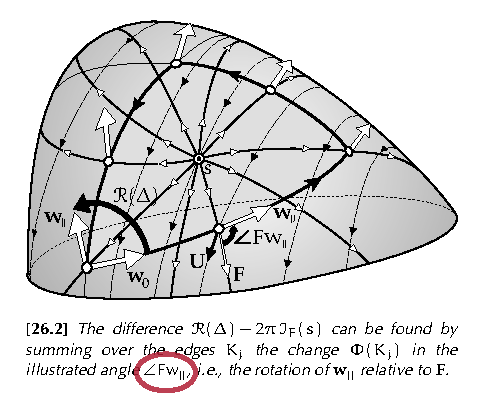
\includegraphics[width=0.9\textwidth]{figs/needham_triangle_circ.pdf}
\caption{{Needham,~T. (2021) Visual Differential Geometry and Forms.}}
\end{figure}
\column{0.5\textwidth}
\vspace{-12pt}
\begin{itemize}
\item The classical proof is discrete-flavored.
\item ``\( \angle Fw_{||} \)'' looked a lot like a pathover.
\item Hopf's \( \Phi \) is defined on edges, not loops. We imitated that too.
\end{itemize}
\end{columns}
\end{frame}
